\documentclass[11pt, a4paper]{article}
\usepackage{pdfpages}
\usepackage{parallel}
\usepackage[T2A]{fontenc}
\usepackage{ucs}
\usepackage[utf8x]{inputenc}
\usepackage[polish,english,russian]{babel}
\usepackage{hyperref}
\usepackage{rotating}
\usepackage[inner=2cm,top=1.8cm,outer=2cm,bottom=2.3cm,nohead]{geometry}
\usepackage{listings}
\usepackage{graphicx}
\usepackage{wrapfig}
\usepackage{longtable}
\usepackage{indentfirst}
\usepackage{array}
\usepackage{tikzsymbols}
\usepackage{soul}
\usepackage[ruled,vlined]{algorithm2e}
%\counterwithout{figure}{section} 

\usepackage{url}
\makeatletter
\g@addto@macro{\UrlBreaks}{\UrlOrds}
\makeatother

\newcolumntype{P}[1]{>{\raggedright\arraybackslash}p{#1}}
\frenchspacing
\usepackage{fixltx2e} %text sub- and superscripts
\usepackage{icomma} % коскі ў матэматычным рэжыме
\PreloadUnicodePage{4}

\newcommand{\longpage}{\enlargethispage{\baselineskip}}
\newcommand{\shortpage}{\enlargethispage{-\baselineskip}}

\def\switchlang#1{\expandafter\csname switchlang#1\endcsname}
\def\switchlangbe{
\let\saverefname=\refname%
\def\refname{Літаратура}%
\def\figurename{Іл.}%
}
\def\switchlangen{
\let\saverefname=\refname%
\def\refname{References}%
\def\figurename{Fig.}%
}
\def\switchlangru{
\let\saverefname=\refname%
\let\savefigurename=\figurename%
\def\refname{Литература}%
\def\figurename{Рис.}%
}

\hyphenation{admi-ni-stra-tive}
\hyphenation{ex-pe-ri-ence}
\hyphenation{fle-xi-bi-li-ty}
\hyphenation{Py-thon}
\hyphenation{ma-the-ma-ti-cal}
\hyphenation{re-ported}
\hyphenation{imp-le-menta-tions}
\hyphenation{pro-vides}
\hyphenation{en-gi-neering}
\hyphenation{com-pa-ti-bi-li-ty}
\hyphenation{im-pos-sible}
\hyphenation{desk-top}
\hyphenation{elec-tro-nic}
\hyphenation{com-pa-ny}
\hyphenation{de-ve-lop-ment}
\hyphenation{de-ve-loping}
\hyphenation{de-ve-lop}
\hyphenation{da-ta-ba-se}
\hyphenation{plat-forms}
\hyphenation{or-ga-ni-za-tion}
\hyphenation{pro-gramming}
\hyphenation{in-stru-ments}
\hyphenation{Li-nux}
\hyphenation{sour-ce}
\hyphenation{en-vi-ron-ment}
\hyphenation{Te-le-pathy}
\hyphenation{Li-nux-ov-ka}
\hyphenation{Open-BSD}
\hyphenation{Free-BSD}
\hyphenation{men-ti-on-ed}
\hyphenation{app-li-ca-tion}

\def\progref!#1!{\texttt{#1}}
\renewcommand{\arraystretch}{2} %Іначай формулы ў матрыцы зліпаюцца з лініямі
\usepackage{array}

\def\interview #1 (#2), #3, #4, #5\par{

\section[#1, #3, #4]{#1 -- #3, #4}
\def\qname{LVEE}
\def\aname{#1}
\def\q ##1\par{{\noindent \bf \qname: ##1 }\par}
\def\a{{\noindent \bf \aname: } \def\qname{L}\def\aname{#2}}
}

\def\interview* #1 (#2), #3, #4, #5\par{

\section*{#1\\{\small\rm #3, #4. #5}}
\ifx\ParallelWhichBox\undefined%
    \addcontentsline{toc}{section}{#1, #3, #4}%
\else%
\ifnum\ParallelWhichBox=0%
    \addcontentsline{toc}{section}{#1, #3, #4}%
\fi\fi%

\def\qname{LVEE}
\def\aname{#1}
\def\q ##1\par{{\noindent \bf \qname: ##1 }\par}
\def\a{{\noindent \bf \aname: } \def\qname{L}\def\aname{#2}}
}

\newcommand{\interviewfooter}[1]{
\vskip 1em
\noindent \textit{#1}
}

\switchlang{ru}
\begin{document}

\title{1986 "--- NEC Crystal mouse}
\date{}
\maketitle
\selectlanguage{russian}
В сентябре 1986 года корпорация NEC анонсировала рабочую станцию EWS 4800, работавшую под управлением ОС UNIX. Эта машина была спроектирована как рабочая станция для инженеров, для повышения эффективности решения таких задач, как разработка программного обеспечения, автоматизированное проектирование, научные и инженерные вычисления, сбор и анализ экспериментальных данных \cite{yt}. Она была оснащена графическим многооконным интерфейсом и большим 20-дюймовым дисплеем разрешения $1280 \times 1024 \times 256$. В комплекте с этой мощной рабочей станцией поставлялась мышь NEC Crystall Mouse (рис. \ref{fig:NECCrystalPic}).

\begin{figure}[h]
    \centering
    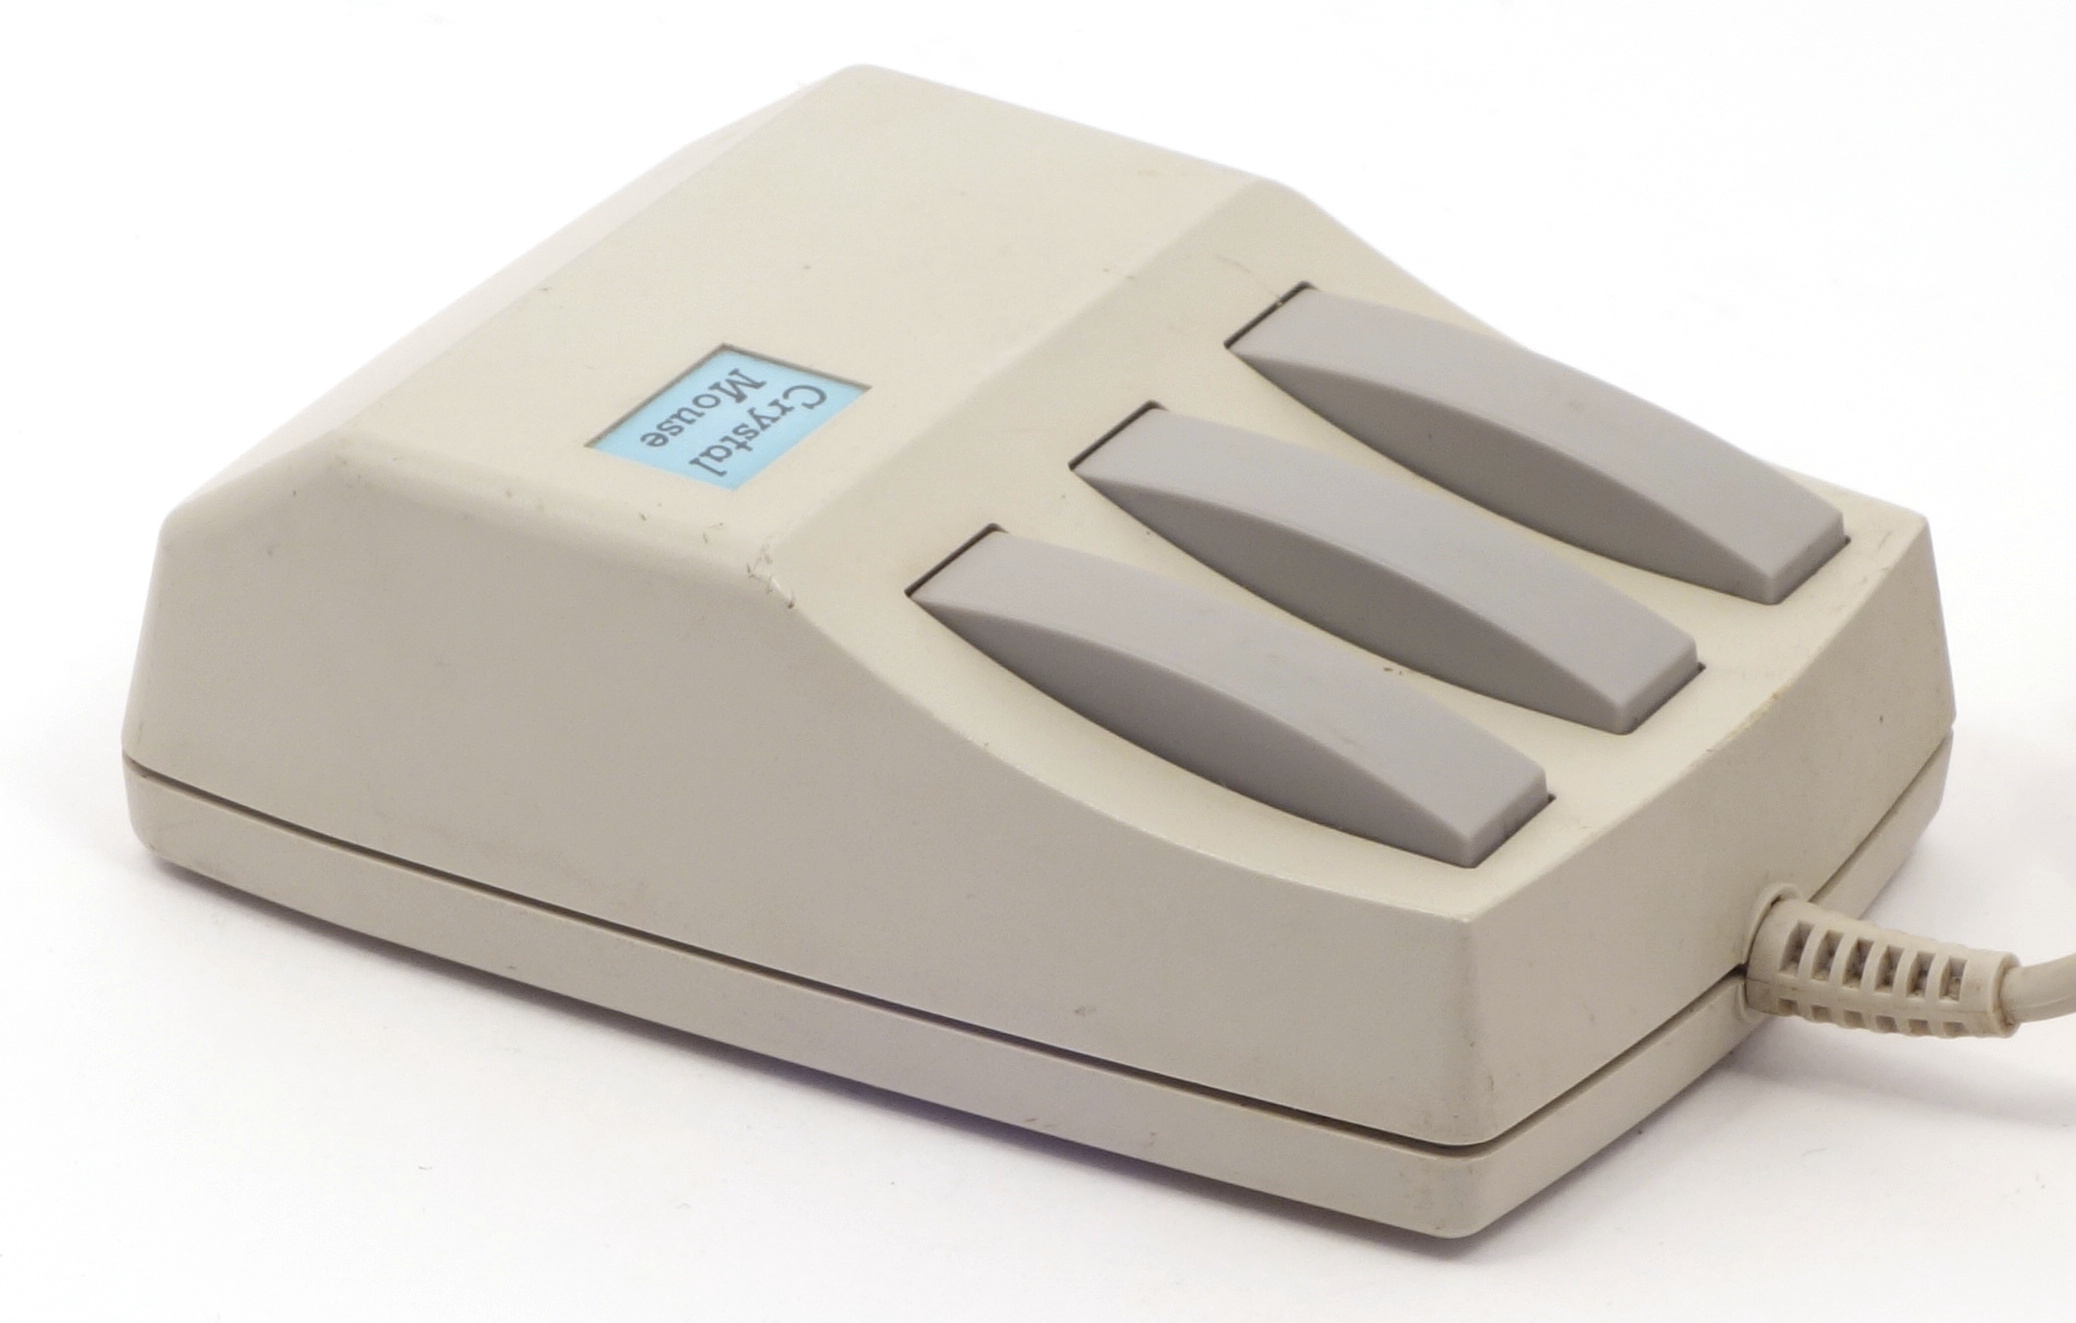
\includegraphics[scale=0.7]{1986_nec_crystal_mouse/necNorm_30.jpg}
    \caption{NEC Crystal Mouse}
    \label{fig:NECCrystalPic}
\end{figure}

На верхней стороне корпуса выделено название мыши <<Crystal Mouse>> с двумя треугольными стилизованными мышками в очертаниях и сплошных линиях. Нижняя сторона показывает, что это оптическая мышь (рис. \ref{NecCrystalTopAndBottom}), во многом повторяющая внешние конструктивные решения мышей Mouse Systems того же периода и предназначенная для использования в комплекте со специальным зеркальным ковриком \cite{photo}.

\begin{figure}[h]
    \centering
    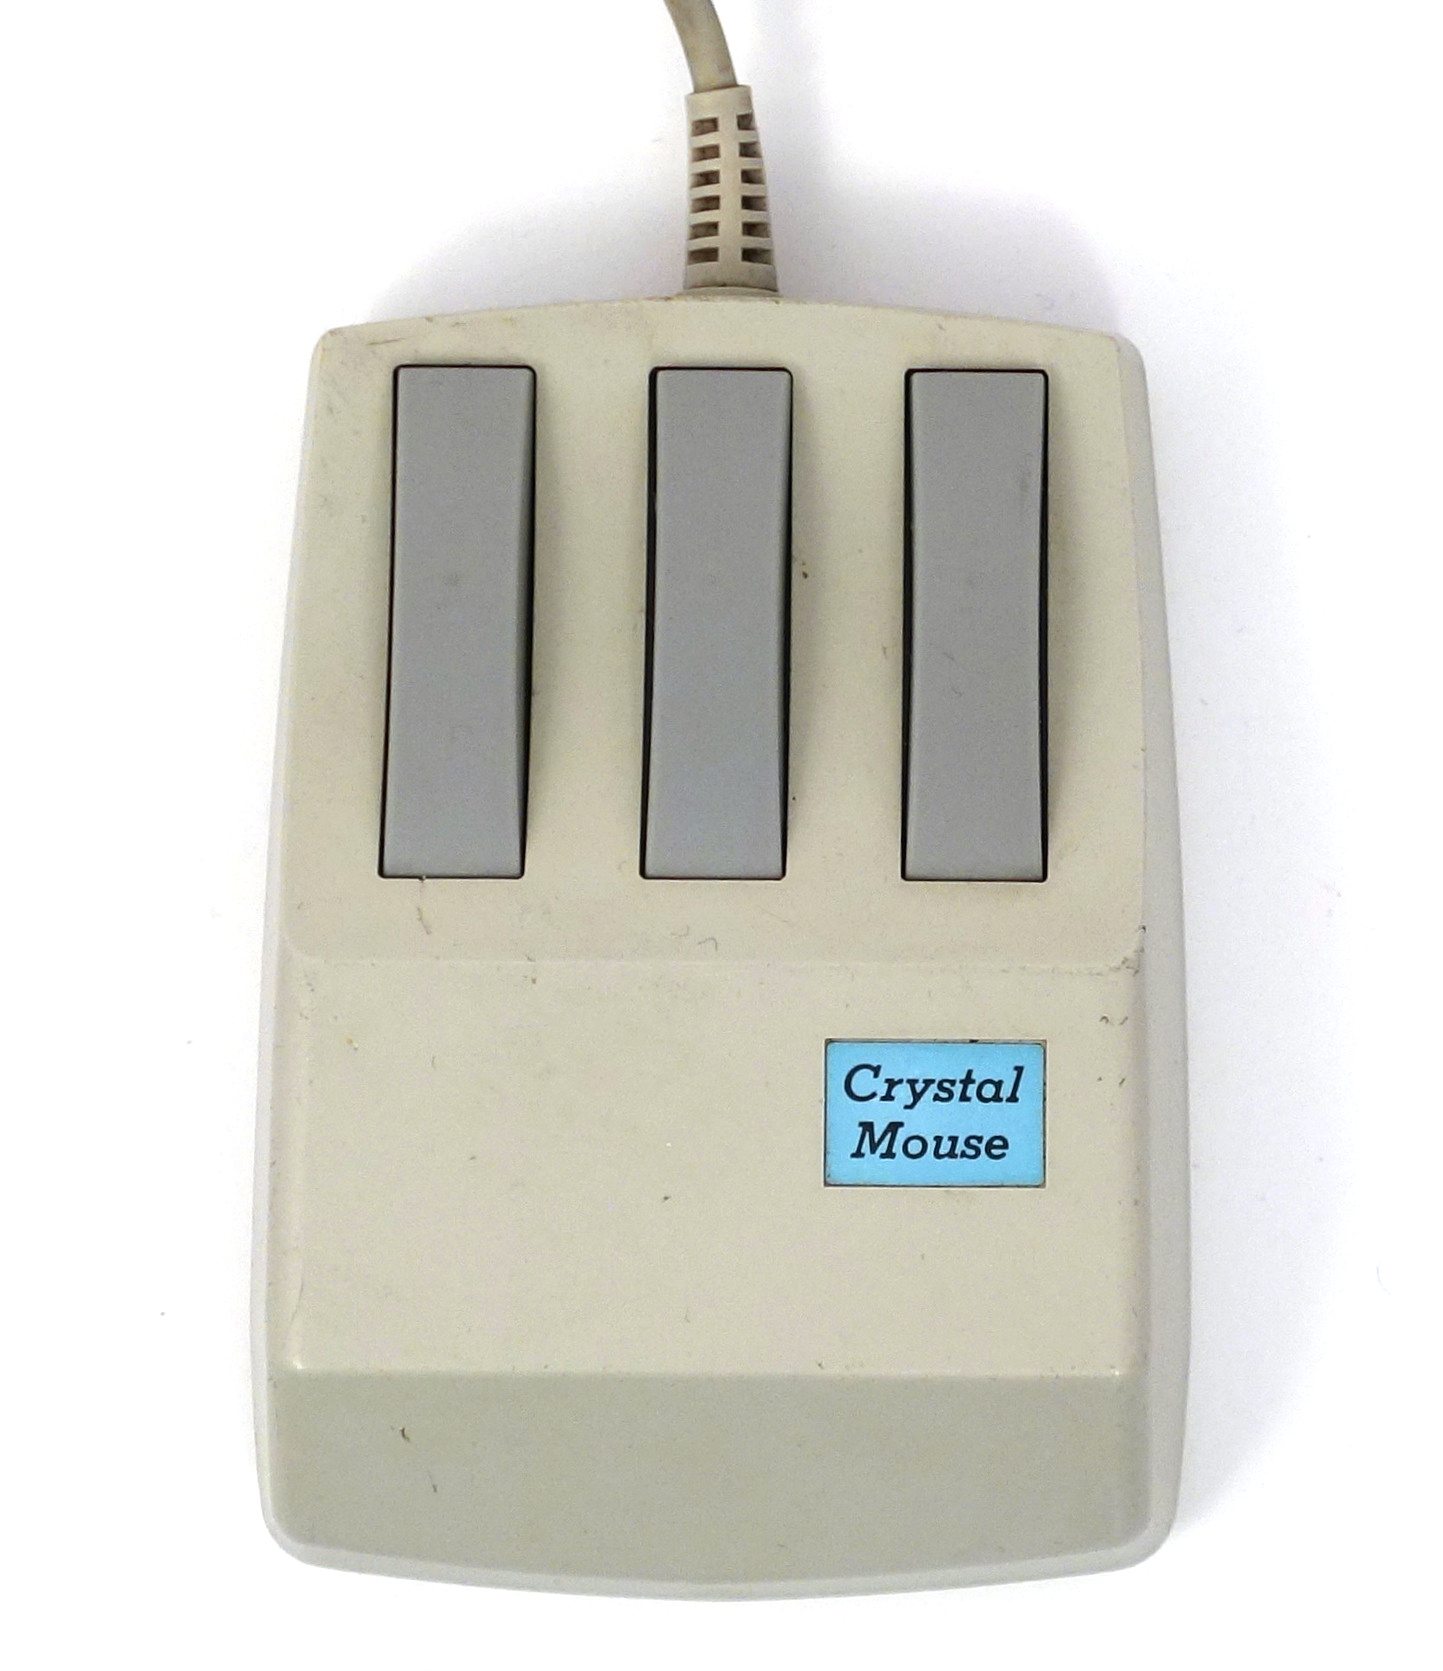
\includegraphics[scale=0.4]{1986_nec_crystal_mouse/nectop_60.jpg}
    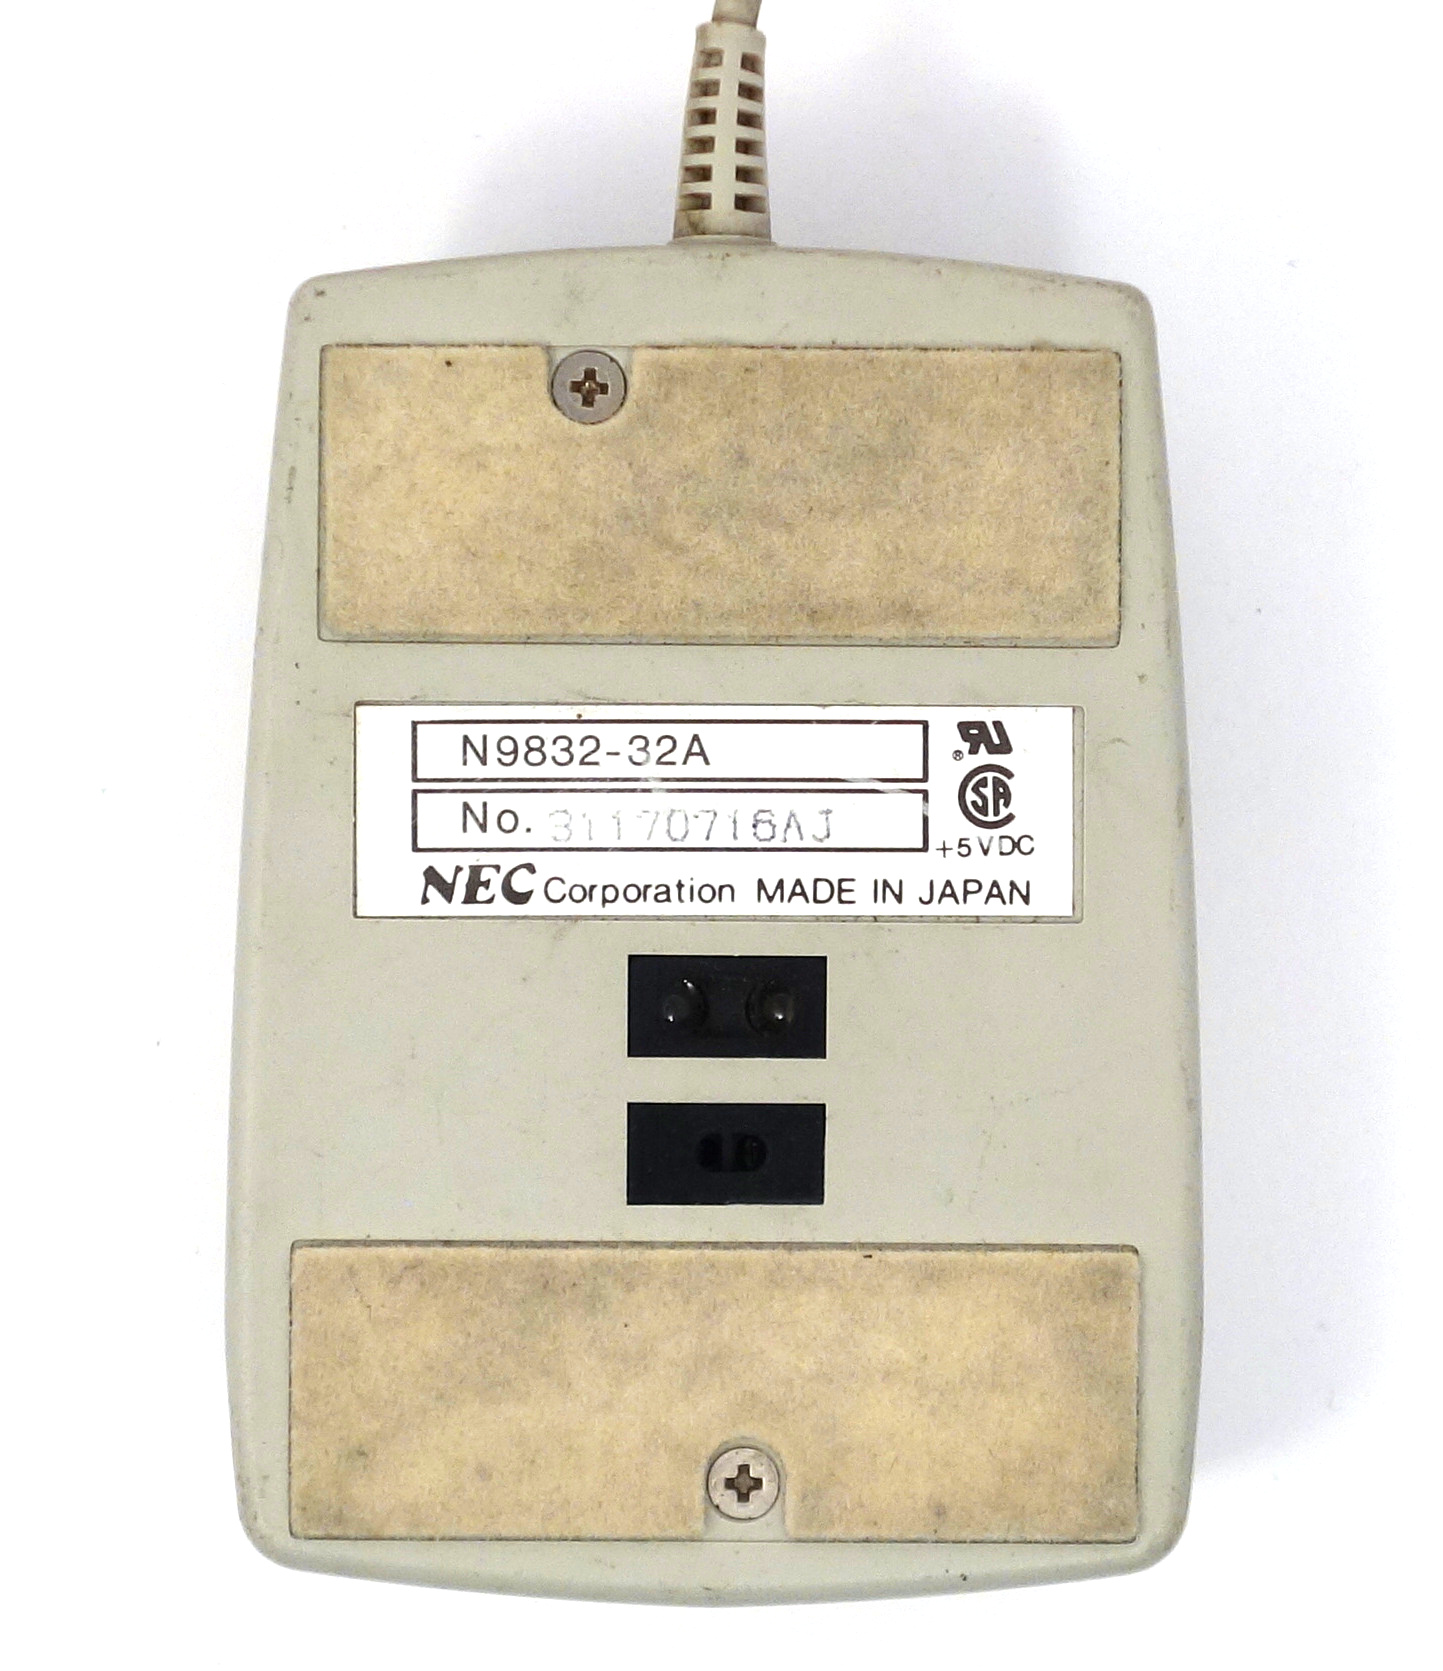
\includegraphics[scale=0.4]{1986_nec_crystal_mouse/necbottom_60.jpg}
    \caption{NEC Crystal Mouse, вид сверху и снизу}
    \label{NecCrystalTopAndBottom}
\end{figure}

В плане размера манипулятор представляет собой типичное для 80-х годов оптическое устройство управления курсором (рис. \ref{fig:NecCrystalSize})

\begin{figure}[h]
    \centering
    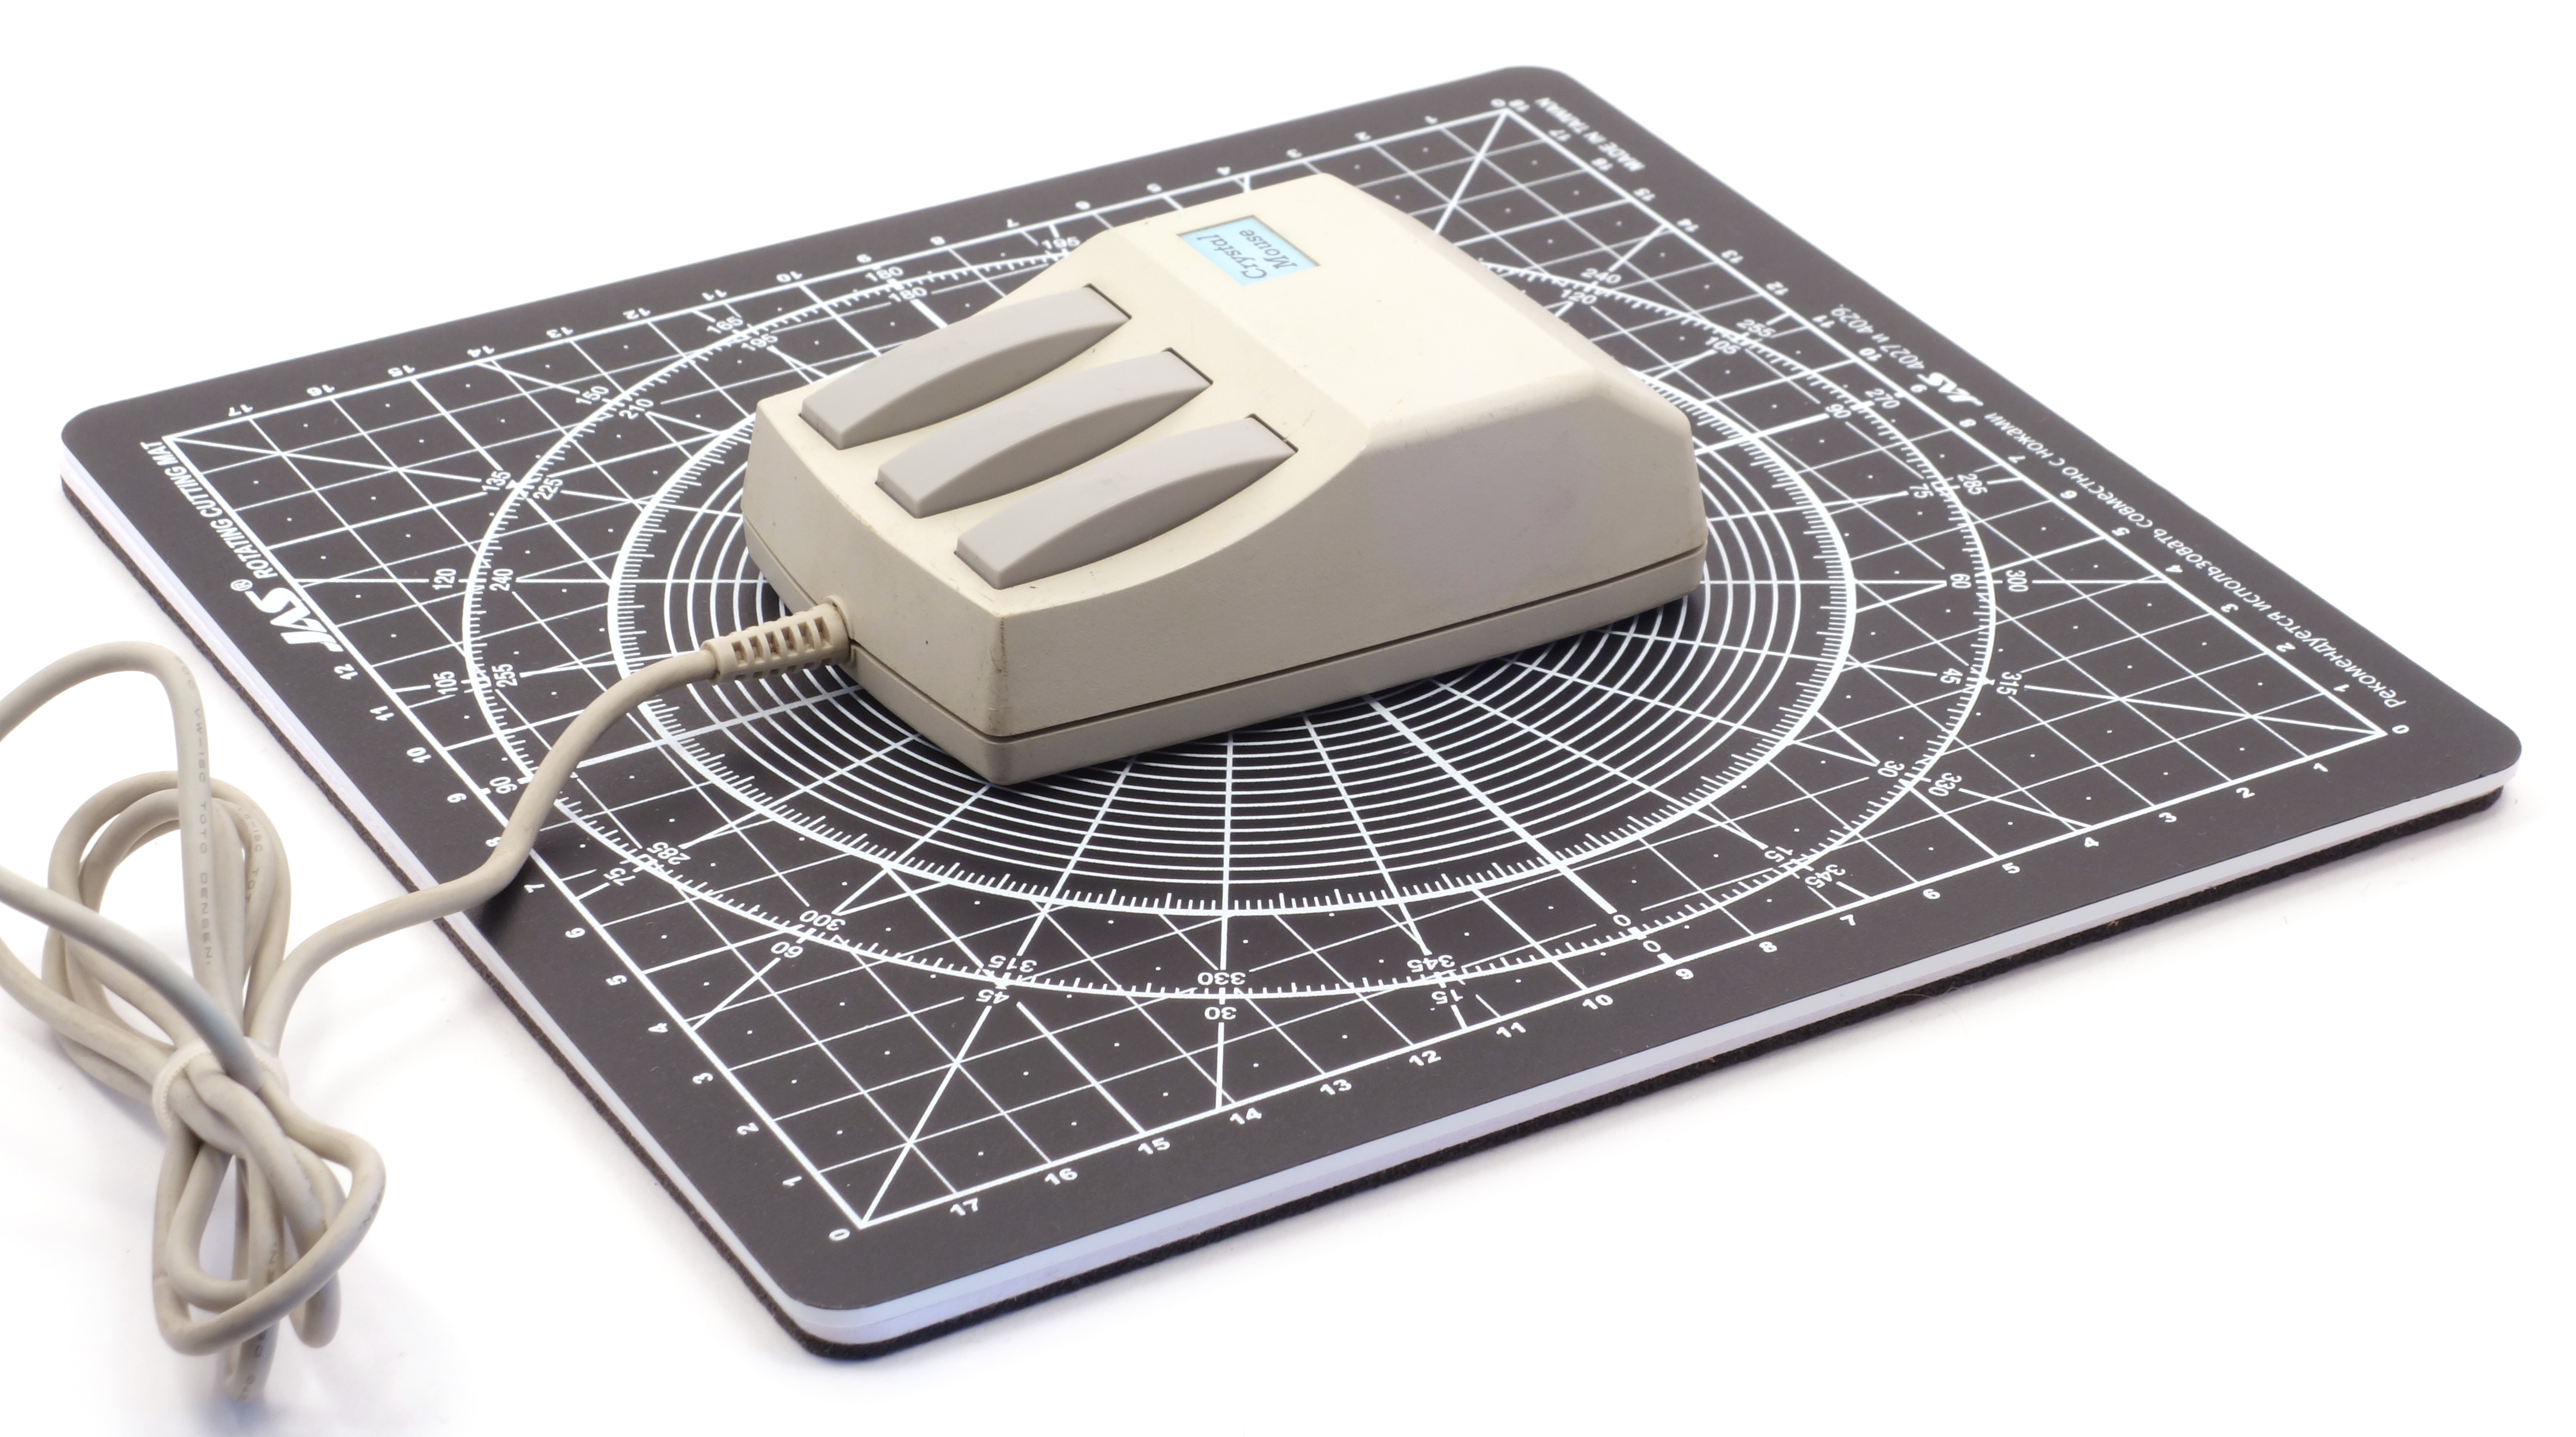
\includegraphics[scale=0.4]{1986_nec_crystal_mouse/NecKovrik_60.jpg}
    \caption{Изображение NEC Crystal Mouse на размерном коврике с шагом сетки 1~см}
    \label{fig:NecCrystalSize}
\end{figure}

В плане эргономики во внешнем виде Crystall Mouse прослеживается ярко выраженный индустриальный дизайн. При этом большое количество углов и плоских граней отчасти компенсируется закругленными стыками граней в ближней к пользователю части корпуса, и выпуклыми продолговатыми кнопками, удобно расположенными в зоне досягаемости пальцев (рис. \ref{fig:NecCrystalHand}).

\begin{figure}[h]
    \centering
    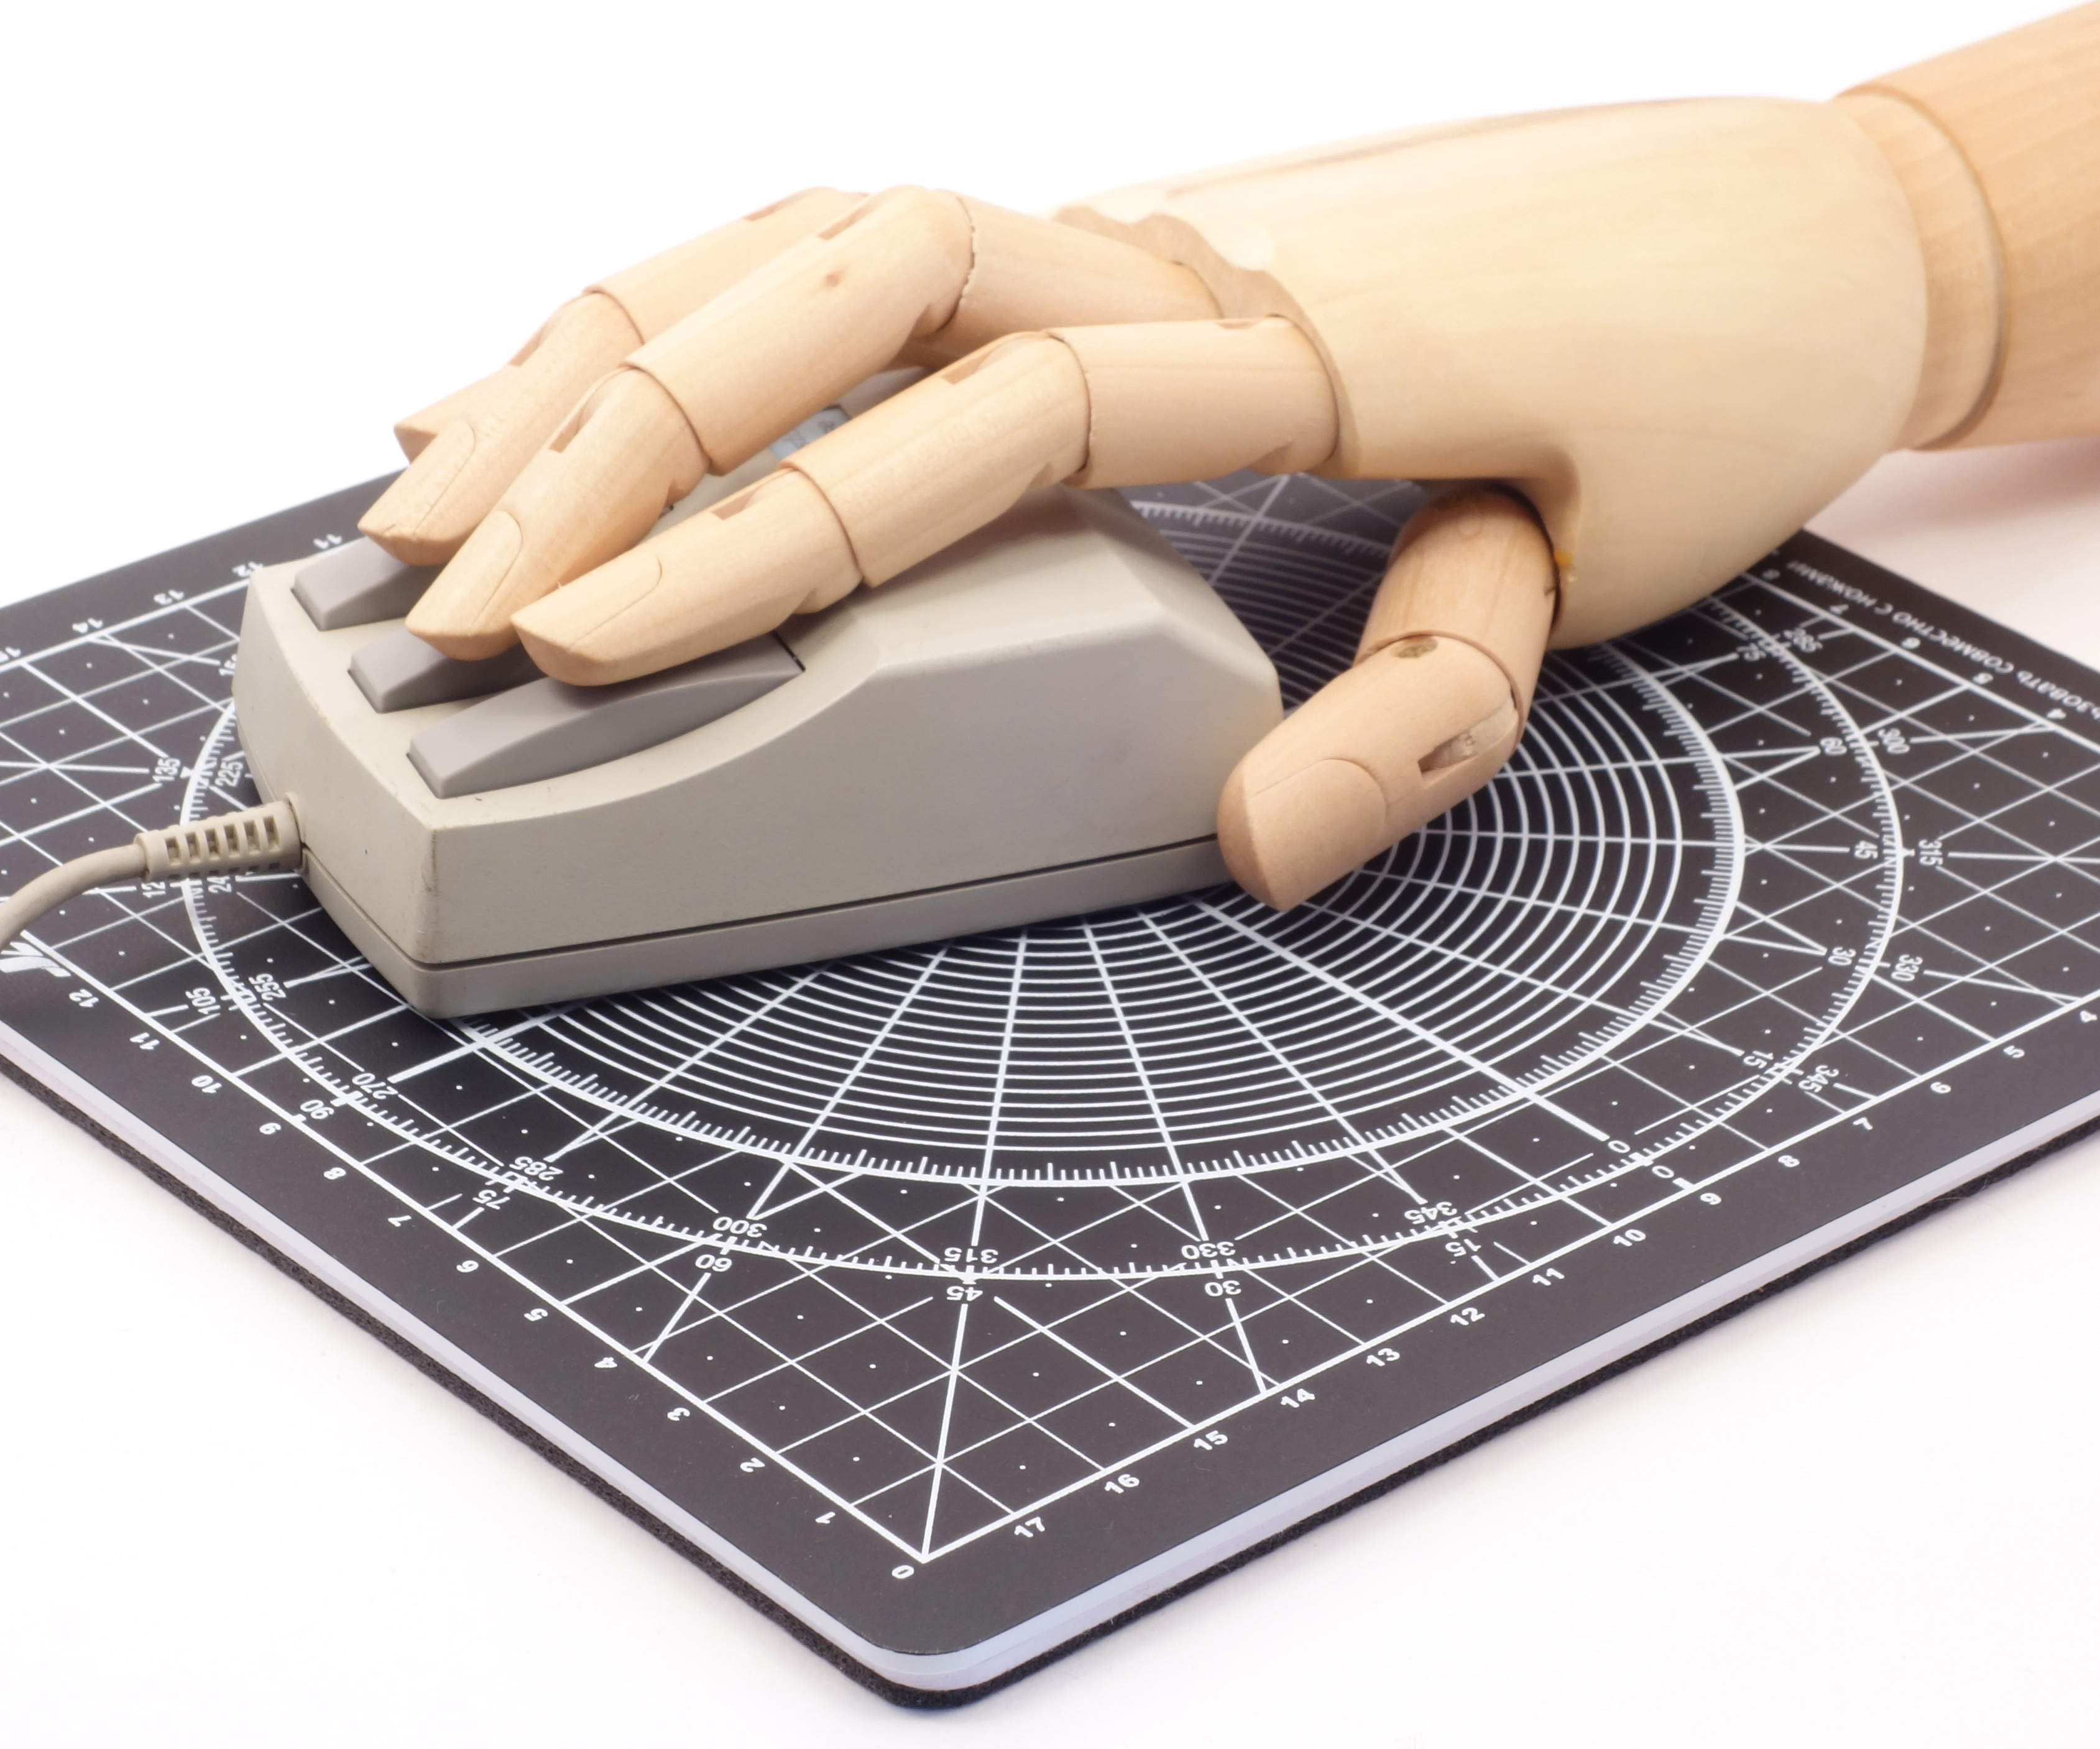
\includegraphics[scale=0.4]{1986_nec_crystal_mouse/NecRuka_30.jpg}
    \caption{NEC Crystal Mouse с моделью руки человека}
    \label{fig:NecCrystalHand}
\end{figure}

NEC Crystall Mouse имеет разъём DIN и по интерфейсу подключения относится к категории Bus Mouse (шинная мышь). Особенностью таких мышей является то, что обработку сигналов оптопар производит не микросхема в корпусе мыши, а специальный адаптер в системном блоке компьютера; поэтому данная мышь питается от компьютера без отдельного блока питания, в отличие от многих ранних оптических моделей, подключавшихся к последовательному порту IBM PC. 

\begin{figure}[h]
    \centering
    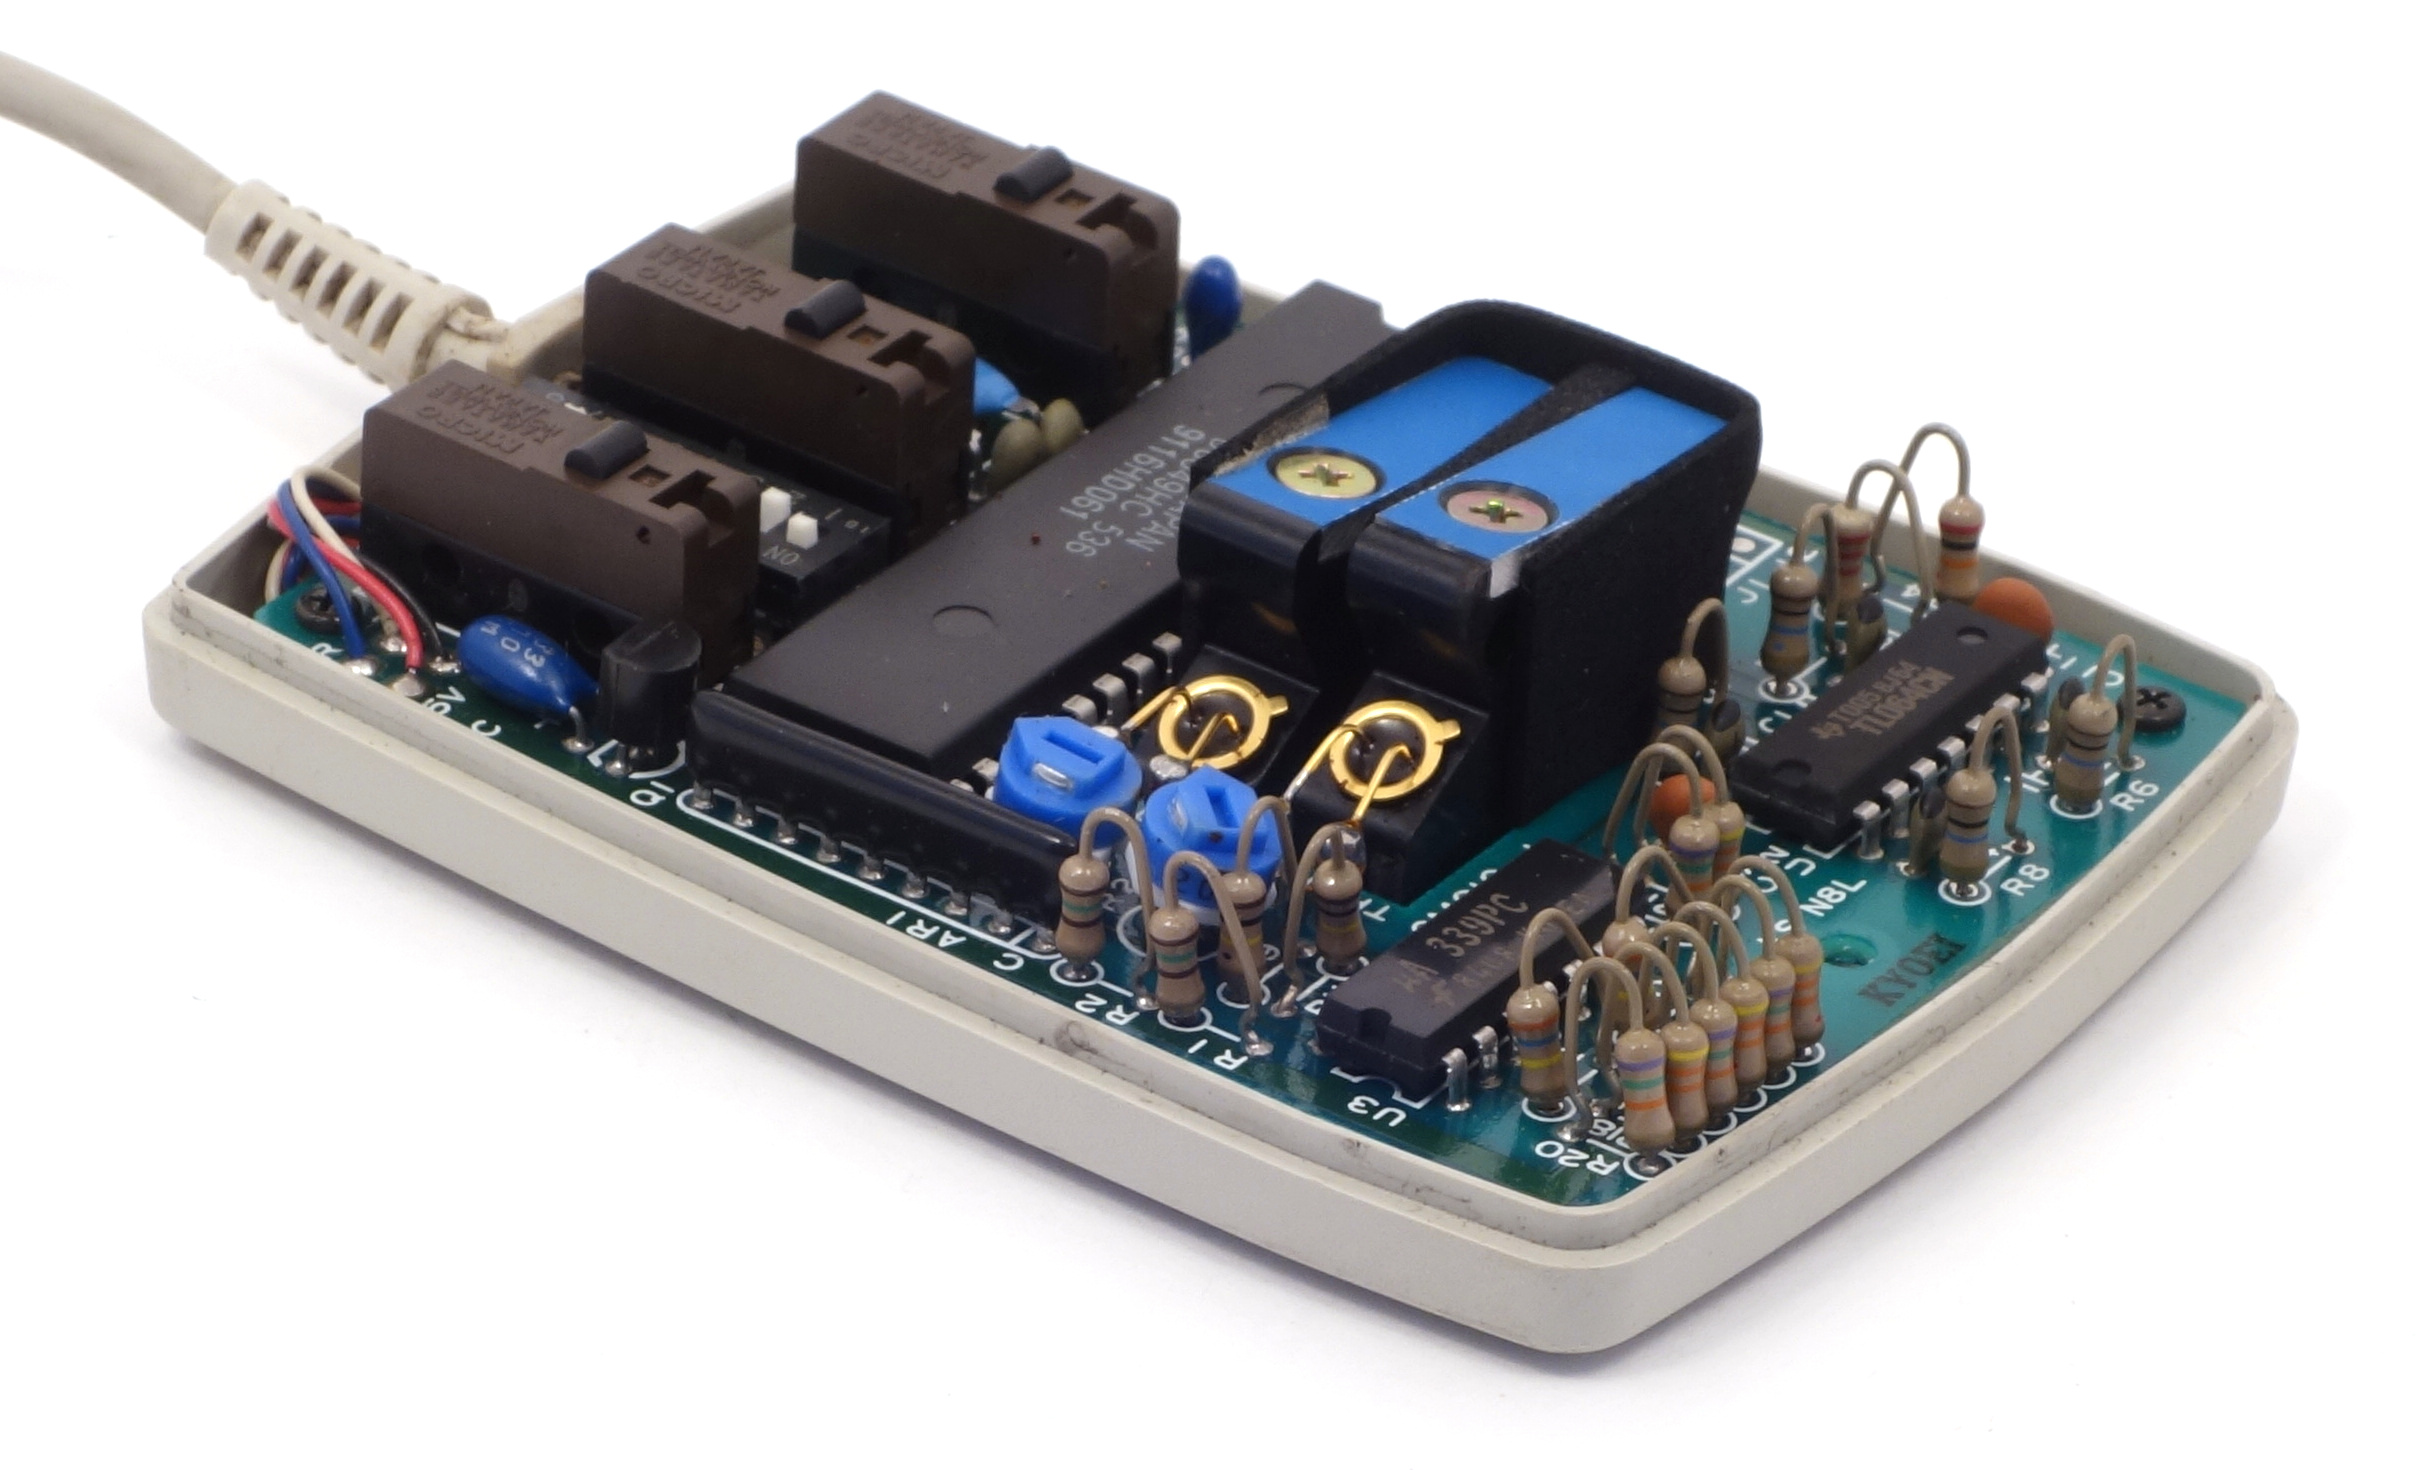
\includegraphics[scale=0.8]{1986_nec_crystal_mouse/necraz_60.jpg}
    \caption{NEC Crystal Mouse в разобранном виде}
    \label{fig:NecCrystalInside}
\end{figure}

В разобранном виде манипулятор показан на рис. \ref{fig:NecCrystalInside}, где можно увидеть оригинальную конструкцию оптической мыши, однако в отличие от большинства оптических мышей 80-х годов, не являющейся прямой копией изделия Mouse Systems, ставшей прототипом для последующих манипуляторов данного типа.
    
\begin{thebibliography}{9}
\bibitem {yt} NEC EWS4800 \url{http://museum.ipsj.or.jp/en/computer/work/0003.html}
\bibitem {photo} Graphics NEC EWS4800 \url{http://www.cs.ce.nihon-u.ac.jp/facility/exp-gazo.html}
\end{thebibliography}
\end{document}
